% Facility Layout and Design -- ALDEP, CORELAP, CRAFT
% Compile from project folder: pdflatex fld_presentation.tex

\documentclass[aspectratio=169,10pt]{beamer}

\usepackage[T1]{fontenc}
\usepackage{lmodern}
\usepackage{graphicx}
\usepackage{booktabs}
\usepackage{amsmath}
\usepackage{ragged2e}

\graphicspath{{./plots/}}

\usetheme{Madrid}
\usecolortheme{default}

% Reduce overflow: slightly narrower effective line width for body text
\setbeamersize{text margin left=0.75cm, text margin right=0.75cm}

% Tighter default list spacing; ragged right helps hyphenation in columns
\setlength{\leftmargini}{1.1em}
\setlength{\labelsep}{0.35em}

\title[FLD Project]{Facility Layout Design Pipeline}
\subtitle{Building layouts with ALDEP and CORELAP, then improving them with CRAFT}
\author{Facility Layout and Design}
\date{\today}

\begin{document}

\begin{frame}
  \titlepage
\end{frame}

\begin{frame}{Outline}
  \tableofcontents
\end{frame}

\section{Problem and Inputs}

\begin{frame}[t]{What problem are we solving?}
  \RaggedRight
  \small
  We have a small factory layout problem. Five departments must be placed on a grid.
  The layout is good when important departments are close to each other.

  \vspace{0.55em}
  \begin{itemize}
    \setlength{\itemsep}{0.35em}
    \item \textbf{Departments:} Machining, Assembly, Tooling, Testing, and Shipping.
    \item \textbf{First task:} Create an initial layout using ALDEP and CORELAP.
    \item \textbf{Second task:} Improve each initial layout using CRAFT.
    \item \textbf{Final comparison:} Which starting method gives the better final cost?
  \end{itemize}
\end{frame}

\begin{frame}[t]{Departments and required space}
  \centering
  \small
  \begin{tabular}{@{}clc@{}}
    \toprule
    ID & Department & Cells \\
    \midrule
    0 & Machining  & 3 \\
    1 & Assembly   & 2 \\
    2 & Tooling    & 1 \\
    3 & Testing    & 2 \\
    4 & Shipping   & 1 \\
    \bottomrule
  \end{tabular}

  \vspace{0.55em}
  \RaggedRight
  \small
  \begin{itemize}
    \setlength{\itemsep}{0.35em}
    \item ``Cells'' means how many grid squares that department must occupy.
    \item A department with 3 cells needs three connected blocks of space.
    \item The same department sizes are used for every method.
  \end{itemize}
\end{frame}

\begin{frame}[t]{REL chart: which departments should be close?}
  \centering
  \small
  \begin{tabular}{@{}lccccc@{}}
    \toprule
    & Machining & Assembly & Tooling & Testing & Shipping \\
    \midrule
    Machining & -- & A & E & I & O \\
    Assembly  & A  & -- & U & X & I \\
    Tooling   & E  & U  & -- & A & E \\
    Testing   & I  & X  & A  & -- & U \\
    Shipping  & O  & I  & E  & U  & -- \\
    \bottomrule
  \end{tabular}

  \vspace{0.6em}
  \RaggedRight
  \footnotesize
  \textbf{Meaning:}
  A = absolutely necessary, E = especially important, I = important,
  O = ordinary closeness, U = unimportant, X = undesirable.

  \medskip
  ALDEP and CORELAP use this chart to decide which departments should be near each other.
\end{frame}

\begin{frame}[t]{Flow matrix: how much movement happens?}
  \centering
  \footnotesize
  \begin{tabular}{@{}lccccc@{}}
    \toprule
    From $\backslash$ To & Machining & Assembly & Tooling & Testing & Shipping \\
    \midrule
    Machining & 0 & 12 & 4 & 9  & 2  \\
    Assembly  & 3 & 0  & 1 & 14 & 11 \\
    Tooling   & 5 & 2  & 0 & 3  & 0  \\
    Testing   & 4 & 6  & 0 & 0  & 8  \\
    Shipping  & 2 & 3  & 0 & 2  & 0  \\
    \bottomrule
  \end{tabular}

  \vspace{0.45em}
  \RaggedRight
  \small
  \begin{itemize}
    \setlength{\itemsep}{0.35em}
    \item Read each value as \textbf{from the row department to the column department}.
    \item A large value means those two departments should ideally be close.
    \item Example: Assembly $\rightarrow$ Testing is 14, so that movement is very important.
  \end{itemize}
\end{frame}

\begin{frame}[t]{Cost function: how do we judge a layout?}
  \RaggedRight
  \small
  Each department is represented by its \textbf{centroid}, which is the average position
  of all cells occupied by that department.

  \vspace{0.55em}
  \[
    C = \sum_{i\neq j} F_{ij}\, d(\mathbf{c}_i,\mathbf{c}_j)
  \]

  \vspace{0.25em}
  \begin{itemize}
    \setlength{\itemsep}{0.35em}
    \item $C$ is the total material handling cost.
    \item $F_{ij}$ is the movement from $i$ to $j$.
    \item $d(\mathbf{c}_i,\mathbf{c}_j)$ is the rectilinear distance between centroids.
    \item Lower $C$ means a better layout.
  \end{itemize}
\end{frame}

\section{Pipeline Overview}

\begin{frame}[t]{Big picture pipeline}
  \RaggedRight
  \small
  The project has one pipeline, but two starting layouts.

  \vspace{0.55em}
  \begin{enumerate}
    \setlength{\itemsep}{0.4em}
    \item Use the input data: department sizes, REL chart, and flow matrix.
    \item Build an initial layout using \textbf{ALDEP}.
    \item Build another initial layout using \textbf{CORELAP}.
    \item Compute the transport cost of both layouts.
    \item Run \textbf{CRAFT} on each layout to reduce the cost.
    \item Compare the final costs and final layouts.
  \end{enumerate}
\end{frame}

\begin{frame}[t]{Algorithm overview of the full pipeline}
  \RaggedRight
  \footnotesize
  \textbf{Input:} department areas, REL chart, flow matrix, grid size.

  \vspace{0.35em}
  \begin{enumerate}
    \setlength{\itemsep}{0.3em}
    \item Create two seed layouts:
      \[
        L_A = \text{ALDEP output}, \qquad L_C = \text{CORELAP output}
      \]
    \item For each seed layout, calculate department centroids.
    \item Calculate starting cost $C$ using the flow matrix and centroid distances.
    \item Try every pairwise department swap.
    \item Pick the swap that gives the largest decrease in $C$.
    \item If a better swap exists, accept it and repeat.
    \item If no swap improves $C$, stop. That layout is a local optimum.
    \item Plot the initial layouts, final layouts, and cost curves.
  \end{enumerate}
\end{frame}

\section{ALDEP}

\begin{frame}[t]{ALDEP: what it does}
  \RaggedRight
  \small
  ALDEP is a \textbf{construction method}. It builds a layout from scratch.

  \vspace{0.55em}
  \begin{itemize}
    \setlength{\itemsep}{0.35em}
    \item It starts with one department.
    \item It chooses the next department using the REL chart.
    \item It places departments one after another using a sweep pattern on the grid.
    \item It tries to keep departments with strong closeness ratings near each other.
  \end{itemize}
\end{frame}

\begin{frame}[t]{Algorithm 1: ALDEP used here}
  \RaggedRight
  \scriptsize
  \textbf{Input:} departments $D$, areas $a_d$, REL matrix, facility width $W=4$, MDP level $I$.\\
  \textbf{Output:} ALDEP layout $L_A$, placement sequence, REL score curve.

  \vspace{0.35em}
  \begin{tabular}{@{}rp{0.86\linewidth}@{}}
    \toprule
    1 & Set grid height $H=\lceil\sum_d a_d/W\rceil$ and create an empty $H\times W$ grid. \\
    2 & Choose the first department randomly from unplaced departments (seed fixed in this run). \\
    3 & \textbf{while} unplaced departments remain \textbf{do} \\
    4 & \quad Split candidates using REL score to current department: below MDP and at/above MDP. \\
    5 & \quad If at/above-MDP set is nonempty, choose candidate with maximum REL score. \\
    6 & \quad Otherwise choose randomly from below-MDP candidates. Append chosen department to sequence. \\
    7 & Place departments in sequence by a serpentine column sweep; fill $a_d$ cells for each department. \\
    8 & After each full department, record REL adjacency score and partial transport cost. \\
    \bottomrule
  \end{tabular}

  \vspace{0.35em}
  \textbf{Termination:} stop when every department has been selected and all required cells are filled
  (or the sweep reaches the grid width).
\end{frame}

\begin{frame}[t]{ALDEP: resulting initial layout}
  \begin{columns}[T,onlytextwidth]
    \begin{column}{0.5\textwidth}
      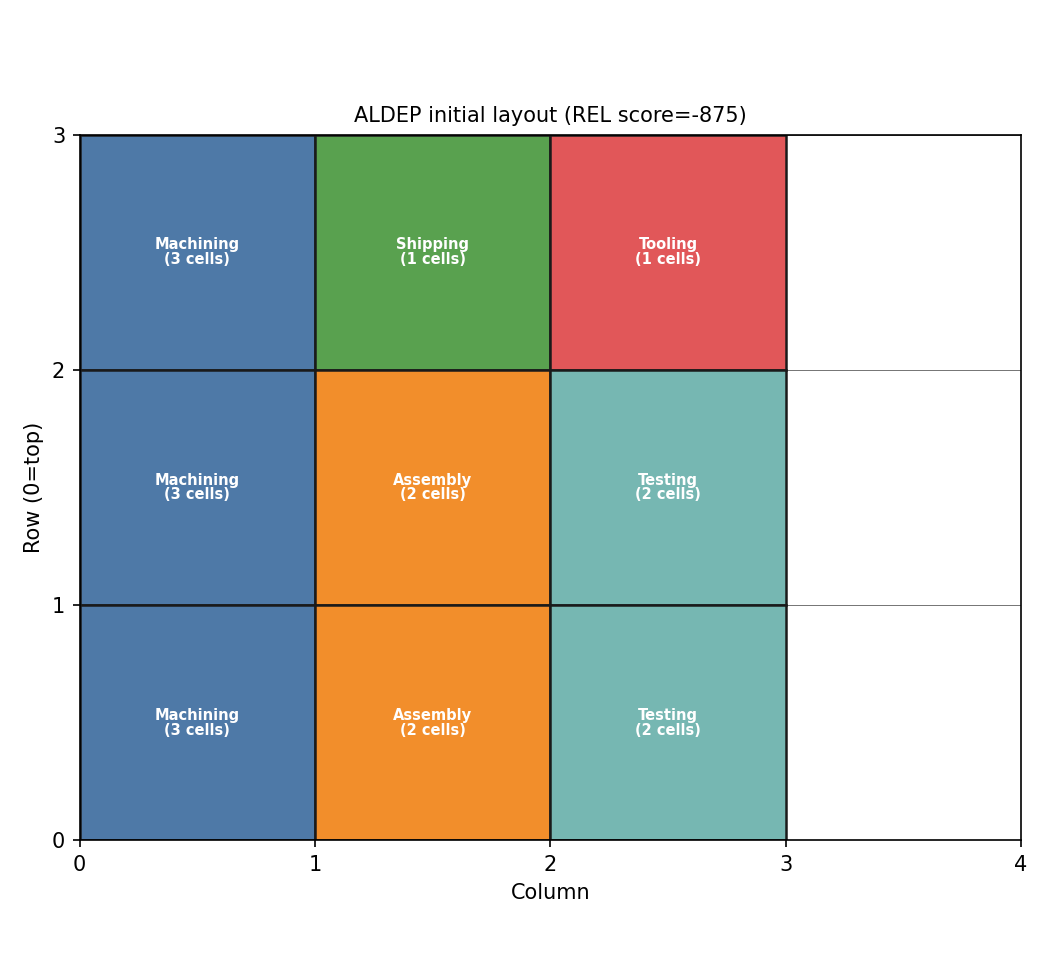
\includegraphics[width=\linewidth,height=0.62\textheight,keepaspectratio]{01_aldep_initial_layout.png}
    \end{column}
    \begin{column}{0.48\textwidth}
      \RaggedRight
      \footnotesize
      This is the first layout produced by ALDEP.

      \medskip
      \textbf{How to read it:}
      Each color is one department. The label shows the department name and the number of cells.

      \medskip
      \textbf{Important:}
      ALDEP focuses on closeness relationships, not directly on transport cost $C$.
    \end{column}
  \end{columns}
\end{frame}

\begin{frame}[t]{ALDEP: progress while building}
  \begin{columns}[T,onlytextwidth]
    \begin{column}{0.52\textwidth}
      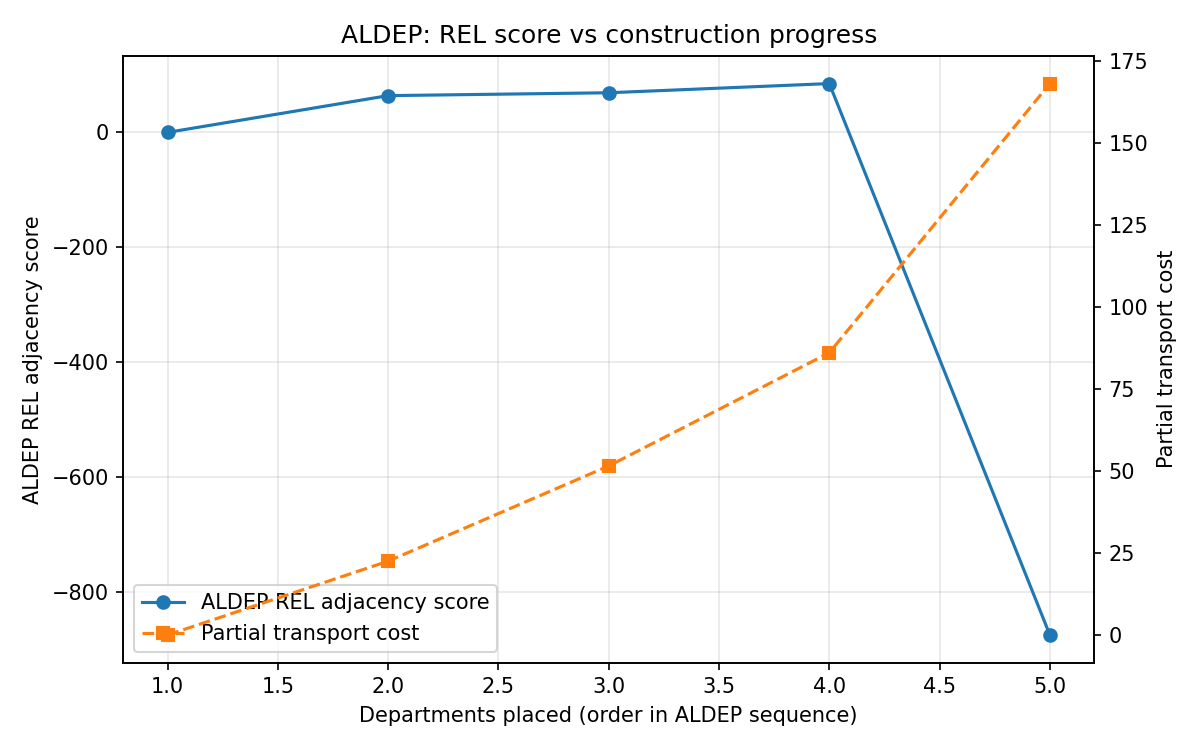
\includegraphics[width=\linewidth,height=0.62\textheight,keepaspectratio]{05_aldep_rel_score_vs_steps.png}
    \end{column}
    \begin{column}{0.46\textwidth}
      \RaggedRight
      \footnotesize
      The graph shows what happens as departments are placed one by one.

      \medskip
      \textbf{Blue line:} REL adjacency score. Higher is better for closeness.

      \medskip
      \textbf{Orange line:} partial transport cost for the departments already placed.

      \medskip
      These two lines may not move together because they measure different things.
    \end{column}
  \end{columns}
\end{frame}

\section{CORELAP}

\begin{frame}[t]{CORELAP: what it does}
  \RaggedRight
  \small
  CORELAP is also a \textbf{construction method}, but it builds the layout differently.

  \vspace{0.55em}
  \begin{itemize}
    \setlength{\itemsep}{0.35em}
    \item First it calculates \textbf{TCR} for each department.
    \item TCR means total closeness rating: how strongly a department wants to be near all others.
    \item The department with high TCR is placed early.
    \item The layout grows outward from the center of the grid.
    \item New cells are chosen where they get the best closeness benefit.
  \end{itemize}
\end{frame}

\begin{frame}[t]{Algorithm 2: CORELAP used here}
  \RaggedRight
  \scriptsize
  \textbf{Input:} departments, sizes, REL chart, $7\times7$ grid.\\
  \textbf{Output:} CORELAP layout $L_C$, placement order, cost curve.

  \vspace{0.35em}
  \begin{tabular}{@{}rp{0.86\linewidth}@{}}
    \toprule
    1 & Compute TCR for each department using weights A=6, E=5, I=4, O=3, U=2, X=1. \\
    2 & Choose first department by maximum TCR; break ties by larger area. \\
    3 & \textbf{while} unplaced departments remain \textbf{do} \\
    4 & \quad For each candidate, find its strongest REL relation to any already placed department. \\
    5 & \quad Choose strongest candidate; break ties by TCR, then area. \\
    6 & Place first block of first department at the grid center. \\
    7 & For each later block, form feasible empty boundary cells: adjacent to layout for a new department, adjacent to same department for extra blocks. \\
    8 & Choose the cell with maximum PR using weights A=243, E=81, I=27, O=9, U=1, X=-729. \\
    \bottomrule
  \end{tabular}

  \vspace{0.35em}
  \textbf{Termination:} stop after every department in the order has received all its required cells.
\end{frame}

\begin{frame}[t]{CORELAP: resulting initial layout}
  \begin{columns}[T,onlytextwidth]
    \begin{column}{0.5\textwidth}
      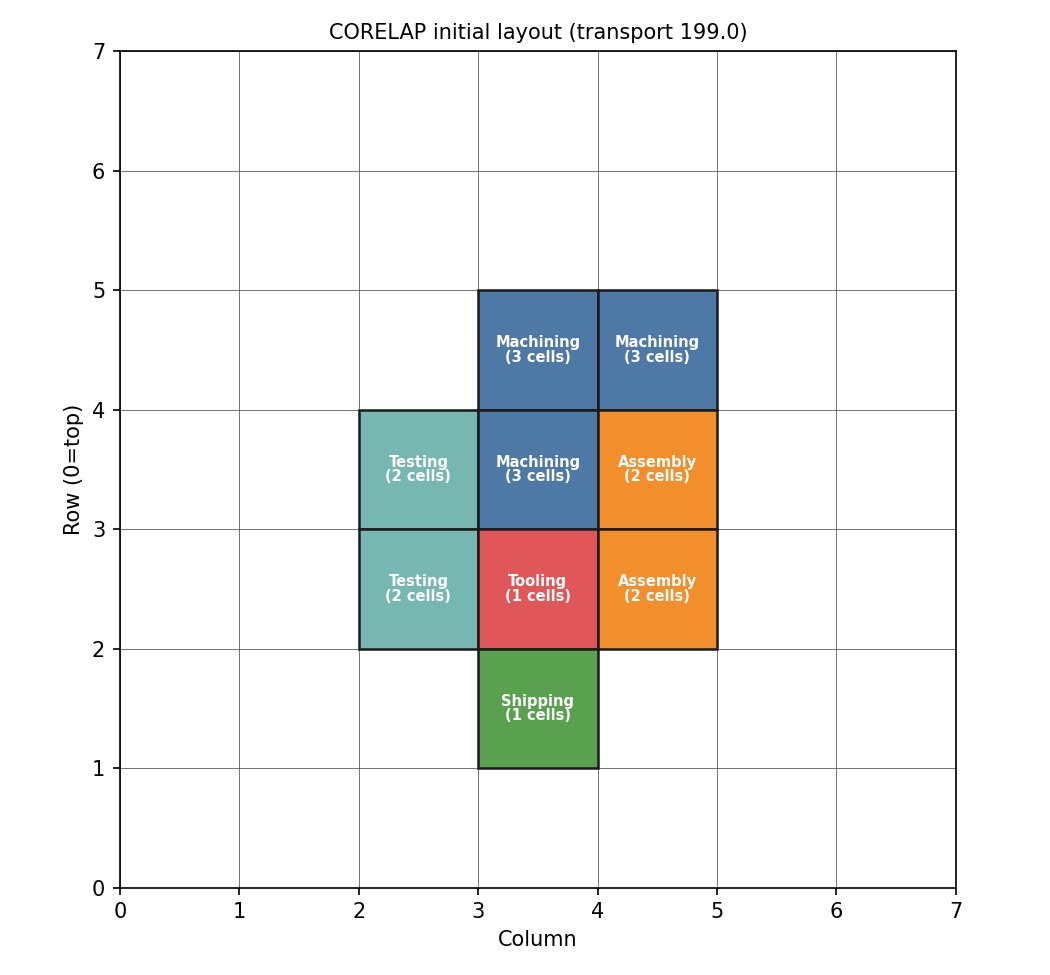
\includegraphics[width=\linewidth,height=0.62\textheight,keepaspectratio]{02_corelap_initial_layout.png}
    \end{column}
    \begin{column}{0.48\textwidth}
      \RaggedRight
      \footnotesize
      This is the first layout produced by CORELAP.

      \medskip
      The same department colors are used as in the ALDEP slide.

      \medskip
      \textbf{Important:}
      CORELAP usually creates a different starting shape because it grows from the center.
    \end{column}
  \end{columns}
\end{frame}

\begin{frame}[t]{CORELAP: transport while building}
  \begin{columns}[T,onlytextwidth]
    \begin{column}{0.52\textwidth}
      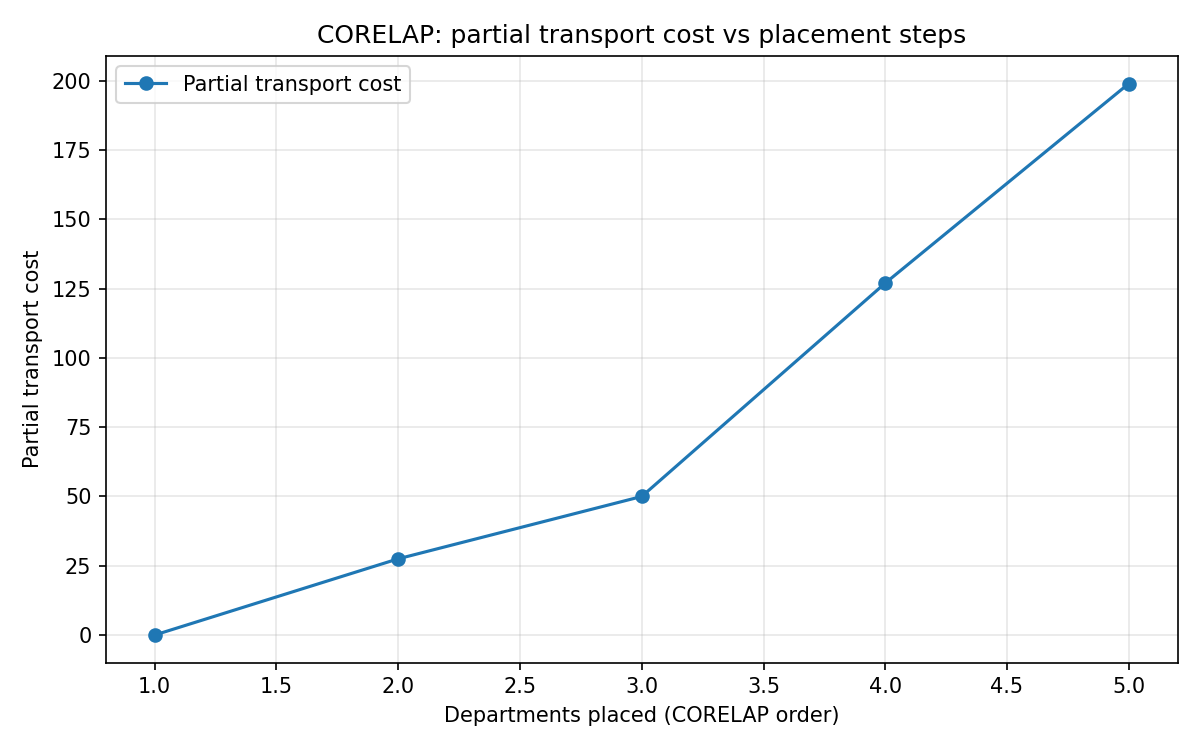
\includegraphics[width=\linewidth,height=0.62\textheight,keepaspectratio]{06_corelap_transport_vs_steps.png}
    \end{column}
    \begin{column}{0.46\textwidth}
      \RaggedRight
      \footnotesize
      This plot shows the transport cost after each full department has been placed.

      \medskip
      The curve can go up or down while building because CORELAP is still constructing
      the layout. It is not yet doing CRAFT improvement.

      \medskip
      The final CORELAP layout becomes the second seed for CRAFT.
    \end{column}
  \end{columns}
\end{frame}

\section{CRAFT}

\begin{frame}[t]{CRAFT: what it does}
  \RaggedRight
  \small
  CRAFT is an \textbf{improvement method}. It does not start from an empty grid.
  It takes an existing layout and tries to make it cheaper.

  \vspace{0.55em}
  \begin{itemize}
    \setlength{\itemsep}{0.35em}
    \item It represents each department by its centroid.
    \item It tries swapping two departments.
    \item It calculates whether the swap reduces total cost $C$.
    \item It accepts the best improving swap.
    \item It repeats until no swap gives a lower cost.
  \end{itemize}
\end{frame}

\begin{frame}[t]{Algorithm 3: CRAFT used here}
  \RaggedRight
  \scriptsize
  \textbf{Input:} seed layout centroids, from-to flow matrix, all department pairs, max iterations $=50$.\\
  \textbf{Output:} improved centroid layout, cost history, accepted swaps.

  \vspace{0.35em}
  \begin{tabular}{@{}rp{0.86\linewidth}@{}}
    \toprule
    1 & Compute current cost $C=\sum_{i\neq j}F_{ij}d(c_i,c_j)$ using rectilinear distance. \\
    2 & Store the current centroid layout in a seen-layout set. \\
    3 & \textbf{for} iteration $=1$ to $50$ \textbf{do} \\
    4 & \quad Evaluate every feasible department pair $(a,b)$ by swapping their centroid coordinates. \\
    5 & \quad For each trial swap, calculate trial cost and gain = current cost $-$ trial cost. \\
    6 & \quad Select the pair with the lowest trial cost, only if it is strictly below current cost. \\
    7 & \quad If no improving pair exists, stop and report ``no improving swap''. \\
    8 & \quad If the new layout has already appeared, stop and report ``cycle detected''. \\
    9 & \quad Otherwise accept the swap, update current layout and cost, and continue. \\
    \bottomrule
  \end{tabular}

  \vspace{0.35em}
  \textbf{Termination:} no improving swap, repeated layout cycle, or 50 iterations reached.
\end{frame}

\begin{frame}[t]{CRAFT after ALDEP}
  \begin{columns}[T,onlytextwidth]
    \begin{column}{0.52\textwidth}
      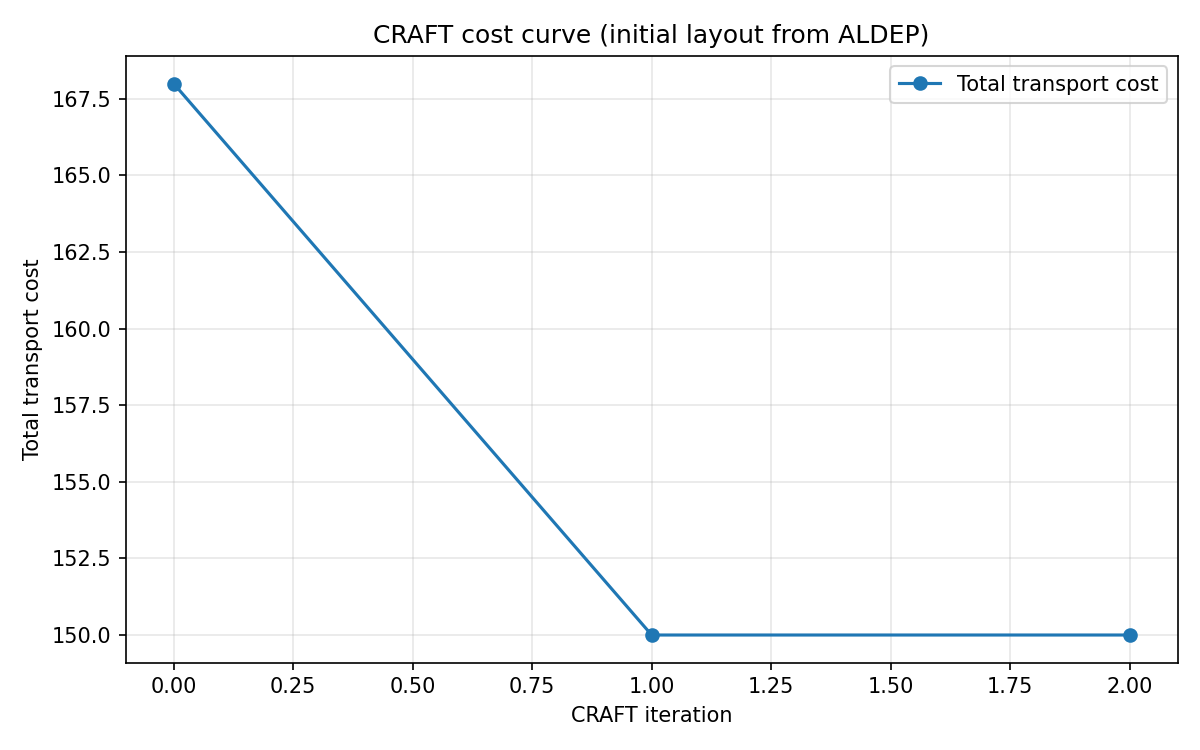
\includegraphics[width=\linewidth,height=0.62\textheight,keepaspectratio]{07_craft_cost_vs_iteration_aldep_seed.png}
    \end{column}
    \begin{column}{0.46\textwidth}
      \RaggedRight
      \footnotesize
      This curve shows how CRAFT improves the ALDEP layout.

      \medskip
      Each drop means CRAFT found a swap that reduced cost.

      \medskip
      When the curve becomes flat, CRAFT cannot find any better swap from that layout.
    \end{column}
  \end{columns}
\end{frame}

\begin{frame}[t]{CRAFT after CORELAP}
  \begin{columns}[T,onlytextwidth]
    \begin{column}{0.52\textwidth}
      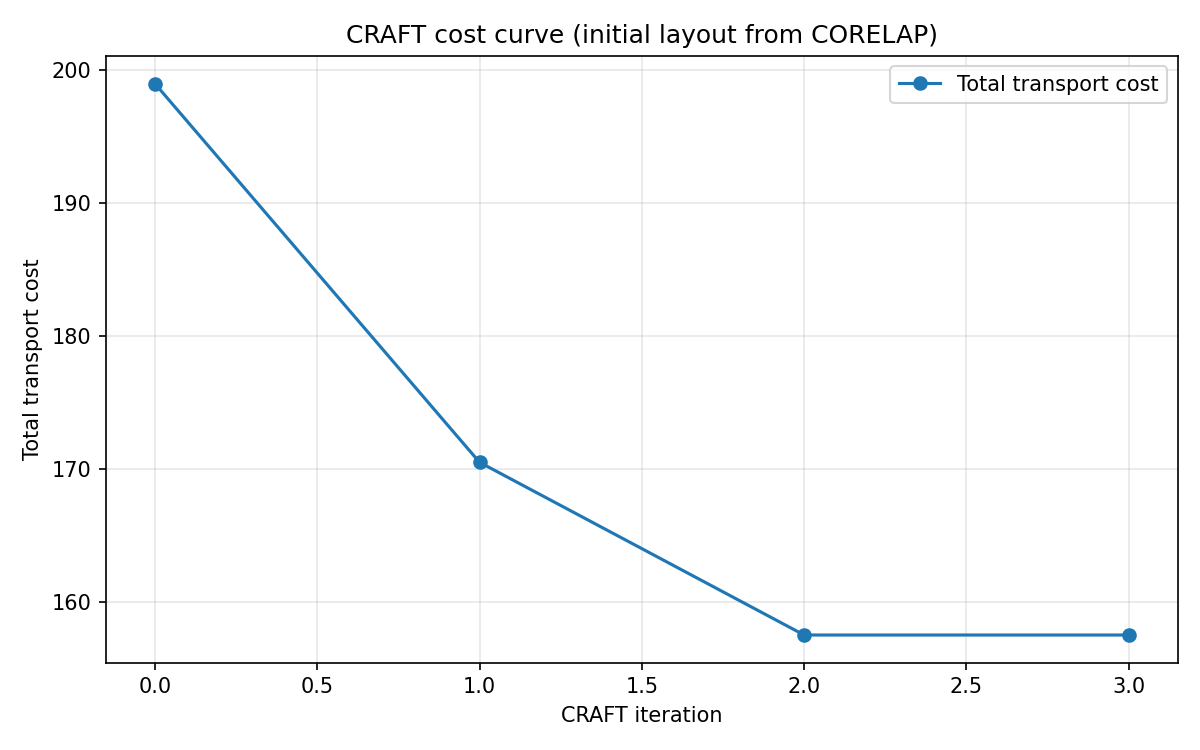
\includegraphics[width=\linewidth,height=0.62\textheight,keepaspectratio]{08_craft_cost_vs_iteration_corelap_seed.png}
    \end{column}
    \begin{column}{0.46\textwidth}
      \RaggedRight
      \footnotesize
      This curve shows how CRAFT improves the CORELAP layout.

      \medskip
      It may follow a different path because the starting layout is different.

      \medskip
      The final point is the best layout CRAFT could reach from the CORELAP seed.
    \end{column}
  \end{columns}
\end{frame}

\begin{frame}[t]{Comparing both CRAFT runs}
  \begin{columns}[T,onlytextwidth]
    \begin{column}{0.49\textwidth}
      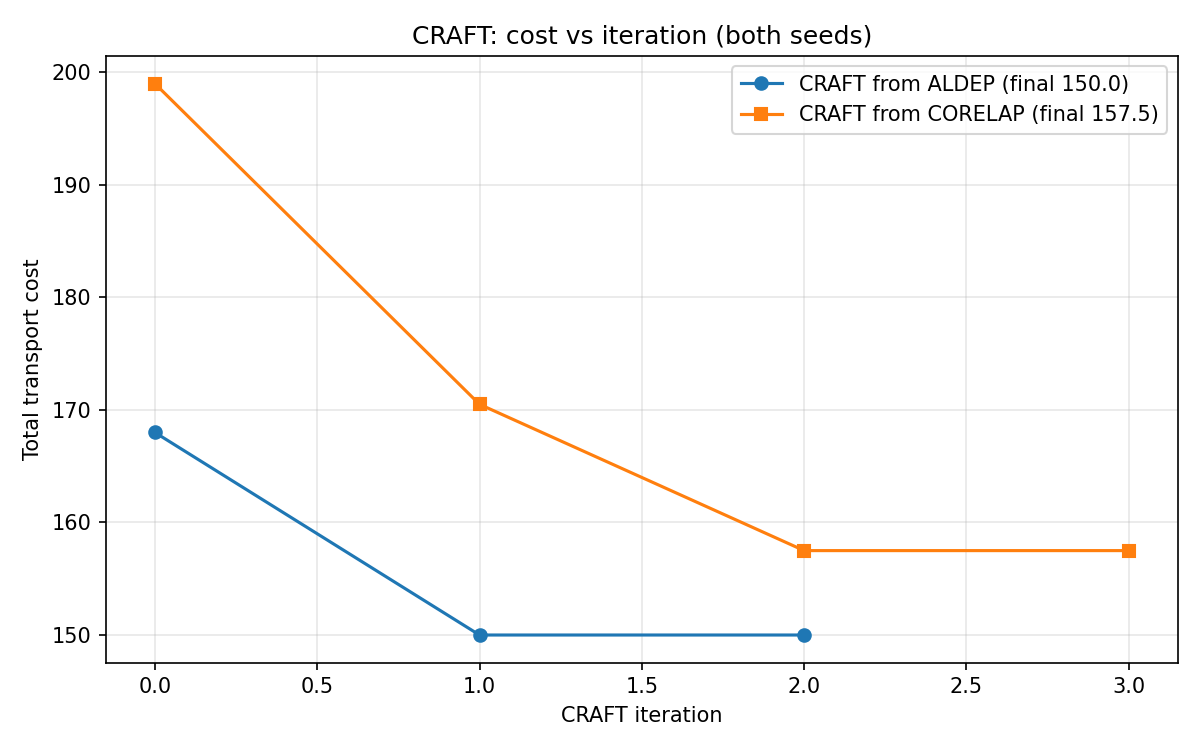
\includegraphics[width=\linewidth,height=0.52\textheight,keepaspectratio]{09_craft_cost_both_seeds.png}
      \par\centering\tiny Both trajectories
    \end{column}
    \begin{column}{0.49\textwidth}
      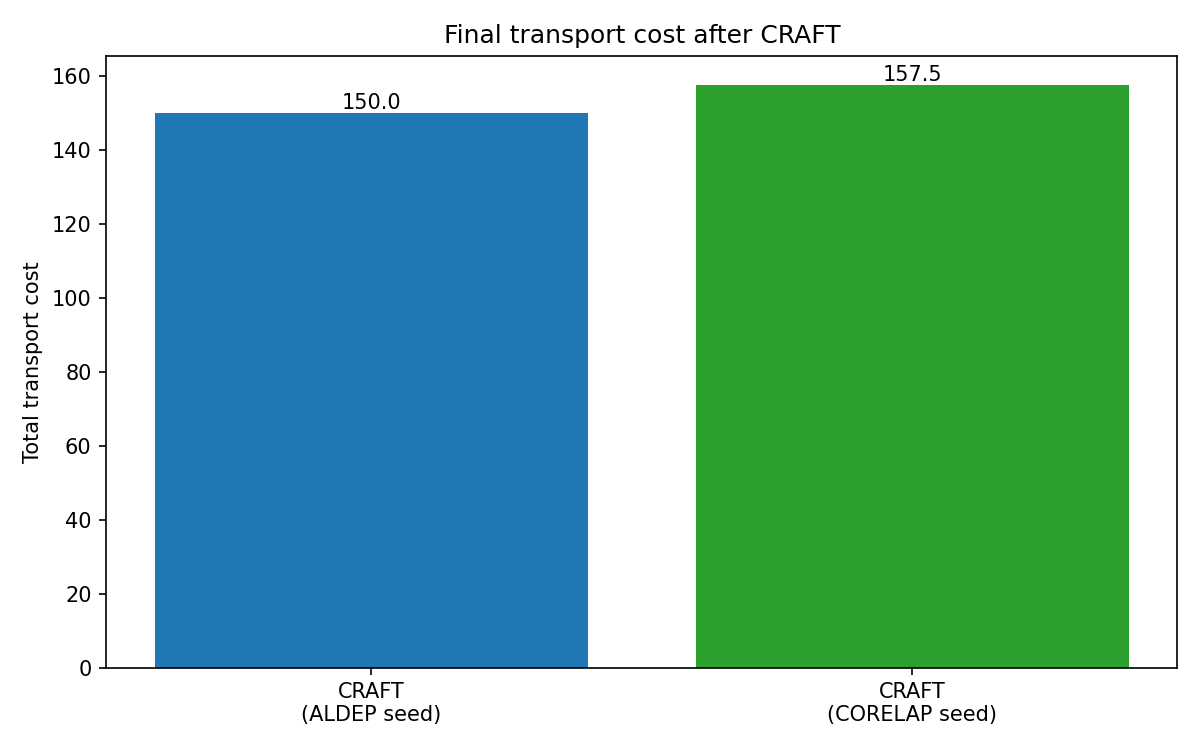
\includegraphics[width=\linewidth,height=0.52\textheight,keepaspectratio]{10_final_cost_comparison.png}
      \par\centering\tiny Final $C$
    \end{column}
  \end{columns}

  \vspace{0.35em}
  \RaggedRight
  \footnotesize
  The line chart compares the improvement path. The bar chart compares the final cost.

  \medskip
  The better final method is the one with the lower final $C$.
\end{frame}

\begin{frame}[t]{Numerical results from the run}
  \centering
  \footnotesize
  \begin{tabular}{@{}lcc@{}}
    \toprule
    Result & ALDEP seed & CORELAP seed \\
    \midrule
    Initial transport cost & 168.00 & 199.00 \\
    CRAFT- cost before swapping & 150.00 & 157.50 \\
    CRAFT- cost after swapping & 168.33 & 180.00 \\
    \bottomrule
  \end{tabular}

  \vspace{0.8em}
  \begin{tabular}{@{}lp{0.68\linewidth}@{}}
    \toprule
    Method & Construction order \\
    \midrule
    ALDEP &
    Machining $\rightarrow$ Assembly $\rightarrow$ Shipping $\rightarrow$ Tooling $\rightarrow$ Testing \\
    CORELAP &
    Machining $\rightarrow$ Assembly $\rightarrow$ Tooling $\rightarrow$ Testing $\rightarrow$ Shipping \\
    \bottomrule
  \end{tabular}

  \vspace{0.6em}
  \RaggedRight
  \scriptsize
  Use the final CRAFT cost to compare ALDEP vs.\ CORELAP. The last row is only a check
  after drawing the accepted swaps back onto grid cells, so it can differ from CRAFT's
  centroid-based cost.
\end{frame}

\begin{frame}[t]{Why post-CRAFT drawings need explanation}
  \RaggedRight
  \small
  CRAFT mainly works with department centroids. But the presentation also shows grid drawings.
  To draw a grid after CRAFT, swaps must be replayed on the actual cells.

  \vspace{0.55em}
  \begin{itemize}
    \setlength{\itemsep}{0.35em}
    \item If two departments have the same area, their cells are exchanged directly.
    \item If areas are different, the smaller department receives the same number of cells it originally had.
    \item The remaining cells stay with the larger department.
  \end{itemize}
\end{frame}

\begin{frame}[t]{How to read post-CRAFT drawings}
  \RaggedRight
  \small
  \begin{itemize}
    \setlength{\itemsep}{0.35em}
    \item The drawings replay the accepted CRAFT swaps in order.
    \item The markers show the geometric centroids after the replay.
    \item The cost curves and bar charts still represent the centroid-based CRAFT model.
    \item Therefore, read the final drawings as a visual explanation of the swaps, not as a new optimization method.
  \end{itemize}
\end{frame}

\begin{frame}[t]{Final layout after CRAFT from ALDEP}
  \begin{columns}[T,onlytextwidth]
    \begin{column}{0.5\textwidth}
      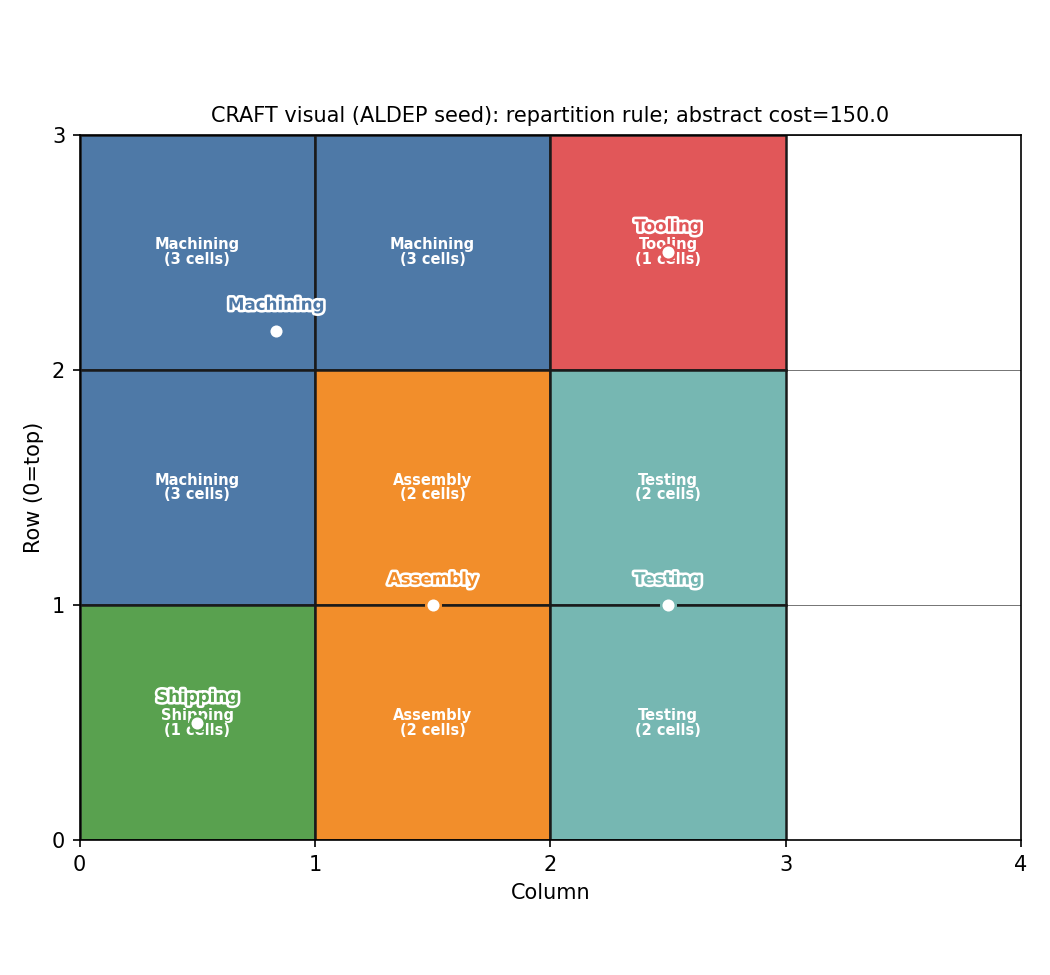
\includegraphics[width=\linewidth,height=0.62\textheight,keepaspectratio]{03_craft_final_from_aldep.png}
    \end{column}
    \begin{column}{0.48\textwidth}
      \RaggedRight
      \footnotesize
      This is the ALDEP starting layout after CRAFT improvements.

      \medskip
      Compare this with the original ALDEP layout. CRAFT has changed department positions
      to reduce transport cost.
    \end{column}
  \end{columns}
\end{frame}

\begin{frame}[t]{Final layout after CRAFT from CORELAP}
  \begin{columns}[T,onlytextwidth]
    \begin{column}{0.5\textwidth}
      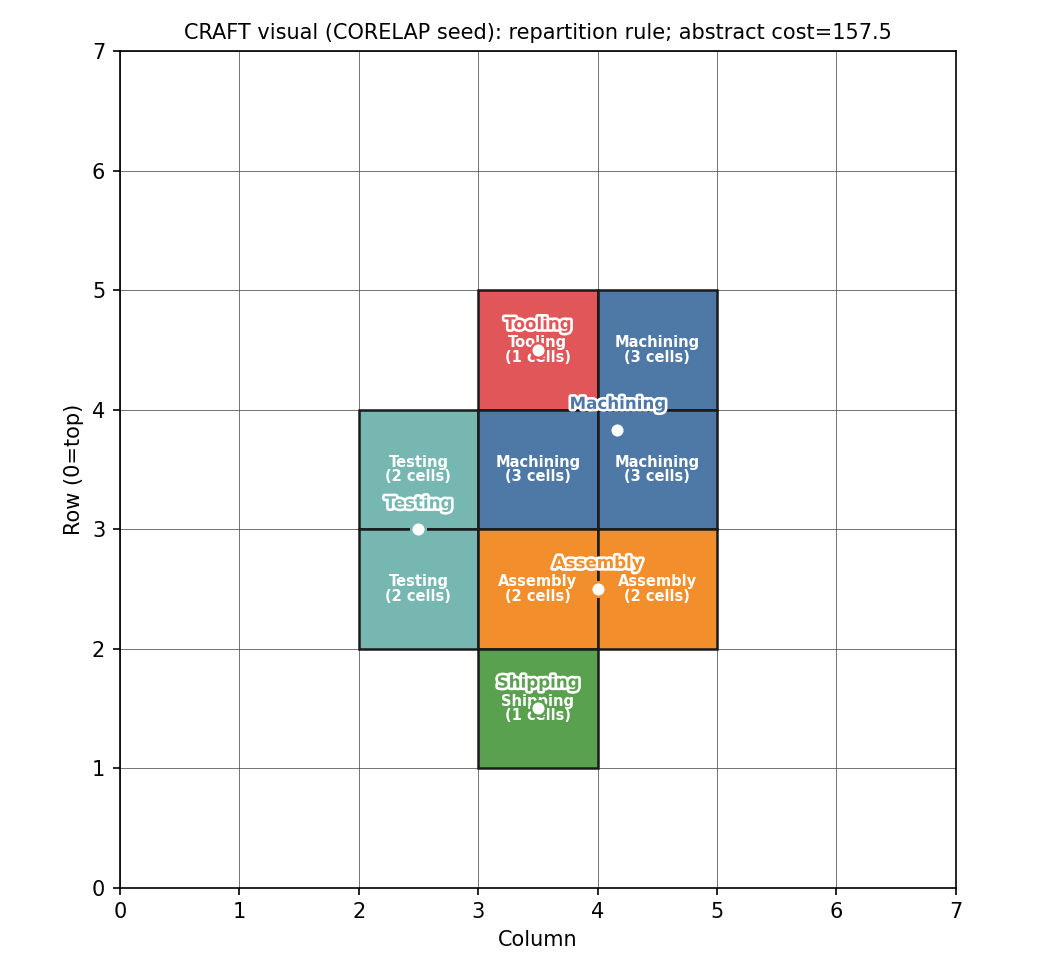
\includegraphics[width=\linewidth,height=0.62\textheight,keepaspectratio]{04_craft_final_from_corelap.png}
    \end{column}
    \begin{column}{0.48\textwidth}
      \RaggedRight
      \footnotesize
      This is the CORELAP starting layout after CRAFT improvements.

      \medskip
      Because the starting layout was different, the final CRAFT layout can also be different.
    \end{column}
  \end{columns}
\end{frame}

\begin{frame}[c]{All four layouts together}
  \centering
  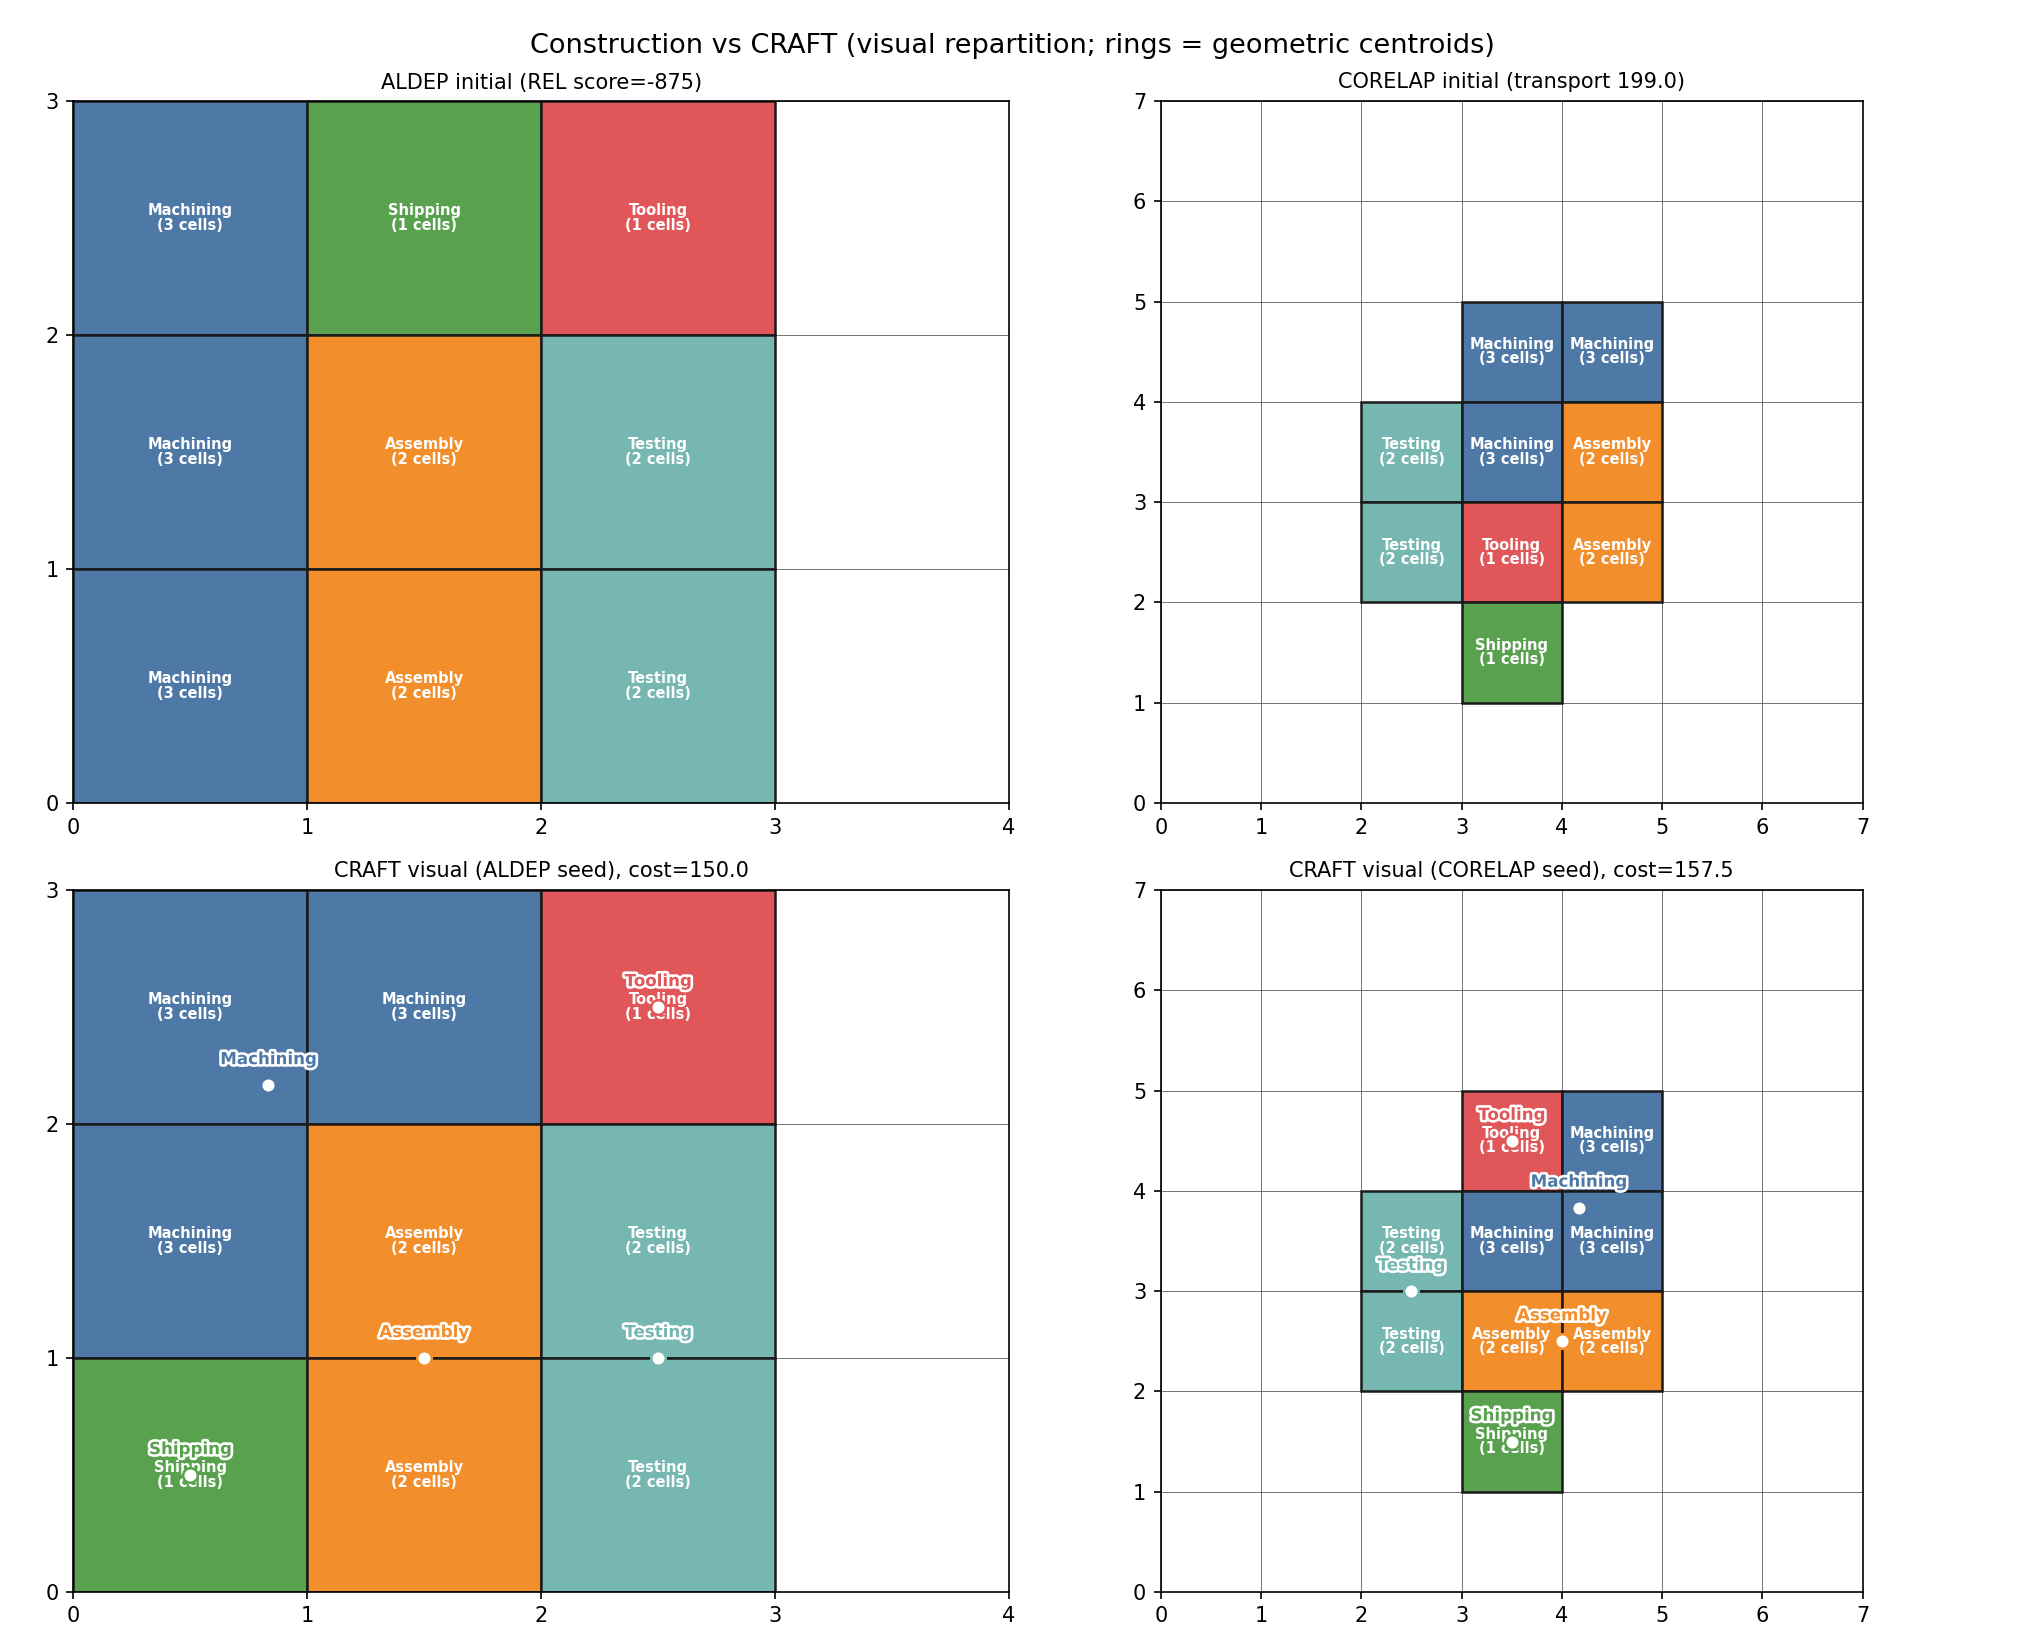
\includegraphics[width=\linewidth,height=0.78\textheight,keepaspectratio]{11_overview_four_panels.png}

  \vspace{0.25em}
  \RaggedRight
  \footnotesize
  Top row: initial layouts from ALDEP and CORELAP.
  Bottom row: final layouts after CRAFT improvement.
\end{frame}

\section{Conclusions}

\begin{frame}[t]{Summary in simple words}
  \RaggedRight
  \small
  \begin{itemize}
    \setlength{\itemsep}{0.35em}
    \item ALDEP and CORELAP are used to create two different initial layouts.
    \item Both methods use closeness information, but they build layouts differently.
    \item CRAFT takes each initial layout and tries to lower material handling cost.
    \item The cost curve shows whether CRAFT is improving the layout.
    \item The final comparison is based on the lower final transport cost $C$.
  \end{itemize}
\end{frame}

\begin{frame}
  \centering
  \Large Thank you for your attention.
\end{frame}

\end{document}
